\section{Ferramentas de Software}
\label{sec:ferramentas}

Esse texto considera 5 ferramentas possíveis para fazer slides acadêmicos, porém na verdade ele se resume a 2 tipos:
\begin{outline}
    \1 ferrramentas WYSIWYG tradicionais
    \2 Power Point, do Microsoft Office
    \2 Slides, da Google
    \2 Impress, do Apache OpenOffice e do LibreOffice
    \2 Keynote, da Apple
    \item \LaTeX\  com \texttt{beamer}
\end{outline}

Existem outras ferramentas para apresentação que buscam métodos menos tradicionais, sendo que possivelmente a mais famosa em 2021 é a Prezi. Uma lista obtida na Internet\footnote{https://visme.co/blog/best-presentation-software/} aponta algumas: Visme, Ludus, Slidebean, Soho Show, Beautiful.ai, Genially, Canva, FlowVella, HaikuDeck e uma ferramenta nova no Microsoft Office chamada Sway.

A maioria dos conselhos dados nesse texto é útil para todas as ferramentas, porém uma ou outra pode exigir uma nova forma de pensar.

\subsection{Power Point}

Se for usar o \textit{Power Point}, use um estilo e o siga. Evite criar caixas soltas de texto, já que os programa fornece estilos próprios. Coloque os textos nos lugares que são indicados pelas caixas de conteúdo.

É fácil usar fórmulas no \textit{Power Point}, tanto dentro do texto quanto em caixas em separado. Porém, cuidado com a portabilidade, já que as fórmulas não navegam bem entre as versões do Power Point, inclusive do Windows para o MacOS acontecem problemas.

Sempre que for trocar de computador, ``\textbf{inclua as fontes ao salvar}''. Isso exige clicar em ``\textit{more options...}'' em vez de no botão salvar e depois clicar em ``\textit{Tools/Save Options}'', novamente em vez de salvar. Aparecerá a opção ``\textit{Embed fonts in the file}'' e, nela, escolha ``\textit{Embed all characters}''.

Se você usar muitas imagens grandes, o arquivo \texttt{.pptx} pode ficar grande demais. Neste caso você pode escolher qualquer imagem e usar o comando \textit{Picture Format/Compress Pictures}. Nesse comando há uma opção que pode ser ligada ou desligada: ``\textit{Apply only to this picture}''. Use-a para comprimir todas as figuras e salvar bastante espaço. Ela permite escolher vários resoluções.

O Power Point permite criar seções. Elas não tem uma grande utilidade, mas podem ser usadas para organizar melhor a visão do \textit{Slide Sorter}. A Figura \ref{fig:sorter} mostra a visão do \textit{Slide sorter}, que é muito útil para visualizar a apresentação como um todo.

\begin{figure}[tbh]
    \centering
    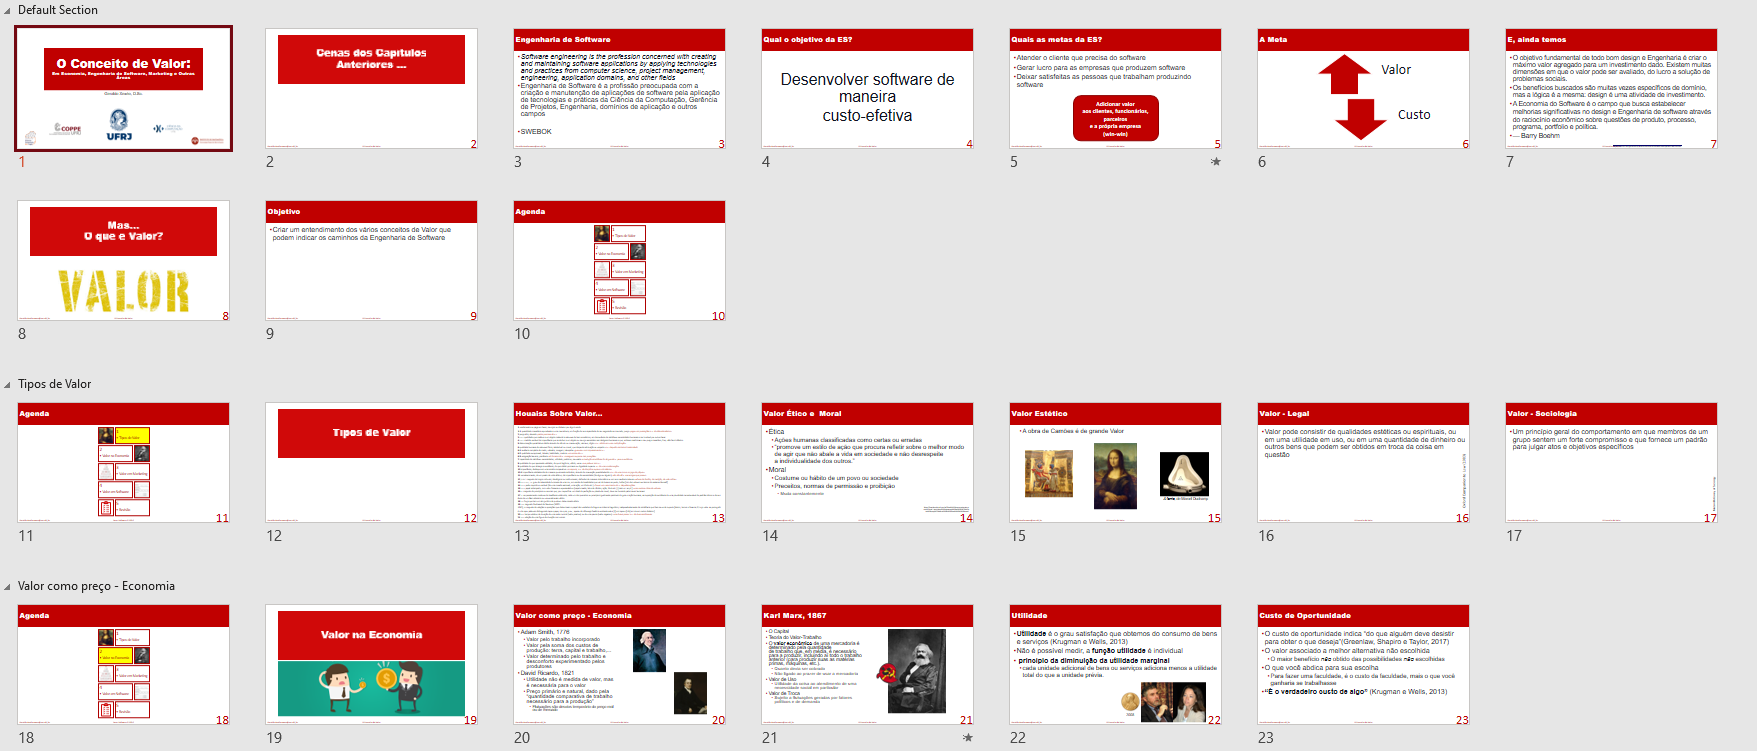
\includegraphics[width=0.7\linewidth]{imagens/slidesorter}
    \caption{Um visão do Slide Sorter do Power Point.}
    \label{fig:sorter}
\end{figure}



\subsection{Google Slides}

Cuidado para não ficar dependente do funcionamento da Internet. Recomendo baixar uma cópia, ou para \textit{Power Point}, ou PDF.

\subsection{\texttt{beamer} e \LaTeX}

Para usuários \LaTeX\ o \texttt{beamer} é uma boa opção. Exemplos de apresentações que fiz com \texttt{beamer} podem ser encontrados em:
\begin{itemize}
    \item \url{https://github.com/xexeo/Seminario-LaTeX-2020}
    \item \url{https://github.com/xexeo/Palestra-Knime}
\end{itemize}

Para usar imagens \texttt{.svg} é necessário ter um software que as processe, eu uso o \textit{InkScape}\footnote{\url{https://inkscape.org/}}.






